% ЕМТ 2024, VII клас — точен LaTeX препис от официалните файлове в Klasirane.com.
% Условия: https://klasirane.com/api/competitions/EMT/All/2024/7%20%D0%BA%D0%BB/probs
% SHA-256 (условия): 6b18c15e6fc854e85d73f901590be08dbbd2b3e3c04a3eed35955d5e8b0693f6
% Решения: https://klasirane.com/api/competitions/EMT/All/2024/7%20%D0%BA%D0%BB/sol
% SHA-256 (решения): 870ef4c3a3e8b1f231ca609212788c043cb632284d80d5b83f46e52ec1b7c319
% Точковите оценки, правописът, формулировките и видимите печатни грешки са запазени от източника.
% Файлът с условията е сканирано изображение; видимите страници са проверени пряко.
% Трите JPEG фигури са извлечени без промяна от официалния PDF с решенията.

Задача 7.1. Фигурите Е и Т на чертежа са съставени от квадратчета със страна 2 cm. Всяка от фигурите се завърта на $360^\circ$ около оста си на симетрия (означена с пунктир) и се получават ротационните тела $P_\mathrm{Е}$ и $P_\mathrm{Т}$.

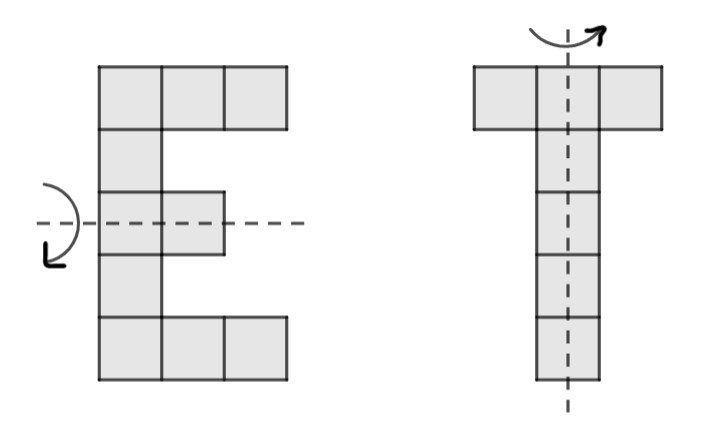
\includegraphics[max width=0.72\textwidth, alt={Фигурите Е и Т и техните оси на симетрия}, center]{assets/7-1-rotations.jpeg}

а) Намерете отношението на лицата на повърхнините на $P_\mathrm{Е}$ и $P_\mathrm{Т}$.

б) Машинни детайли с формата и размерите на $P_\mathrm{Е}$ и $P_\mathrm{Т}$ се отляти от метална сплав. Намерете съответната им маса, като използвате, че 1 cm$^3$ от сплавта тежи 7 g и приемете, че $\pi\approx\dfrac{22}{7}$.

Решение. а) Повърхнината на $P_\mathrm{Е}$ се състои от: околната повърхнина на цилиндър с $r=5$ cm, $h=6$ cm; околната повърхнина на цилиндър с $r=3$ cm, $h=4$ cm; околната повърхнина на цилиндър с $r=1$ cm, $h=2$ cm; кръг с $r=5$ cm; кръг с $r=1$ cm и два кръгови венеца, които общо съставят кръг с $r=5$ cm. Следователно
$$
S_\mathrm{Е}=2\pi.5.6+2\pi.3.4+2\pi.1.2+2.\pi.5^2=138\pi\text{ cm}^2.
$$
Повърхнината на $P_\mathrm{Т}$ се състои от: околната повърхнина на цилиндър с $r=3$ cm, $h=2$ cm; околната повърхнина на цилиндър с $r=1$ cm, $h=8$ cm; кръг с $r=3$ cm; кръг с $r=1$ cm и кръгов венец, които общо съставят кръг с $r=3$ cm. Следователно
$$
S_\mathrm{Т}=2\pi.3.2+2\pi.1.8+2\pi.3^2=46\pi\text{ cm}^2.
$$
Намираме $S_\mathrm{Е}:S_\mathrm{Т}=138\pi:46\pi=3:1$.

б) Обемът на $P_\mathrm{Е}$ се получава, като се съберат обемите на цилиндър с $r=5$ cm, $h=6$ cm и на цилиндър с $r=1$ cm, $h=2$ cm и се извади обемът на цилиндър с $r=3$ cm, $h=4$ cm, т.е.
$$
V_\mathrm{Е}=\pi.5^2.6+\pi.1^2.2-\pi.3^2.4=116\pi\text{ cm}^3.
$$
Тогава масата на $P_\mathrm{Е}$ е приблизително $116\cdot\dfrac{22}{7}\cdot7=2552$ g.

Обемът на $P_\mathrm{Т}$ се се получава, като се съберат обемите на цилиндър с $r=3$ cm, $h=2$ cm и на цилиндър с $r=1$ cm, $h=8$ cm, т.е.
$$
V_\mathrm{Т}=\pi.3^2.2+\pi.1^2.8=26\pi\text{ cm}^3.
$$
Тогава масата на $P_\mathrm{Т}$ е приблизително $26\cdot\dfrac{22}{7}\cdot7=572$ g.

Оценяване. а) Пълно решение: 3 точки.

б) Пълно решение: 3 точки.

Задача 7.2. Намерете всички двойки естествени числа $(p;q)$, за които
$$
p^2-q^2=M,
$$
където
$$
M=\frac{12^{p-2q}\cdot75^{6+6q-3p}}{18^{2p-4q-3}\cdot15^{11-6p+12q}}.
$$

Решение. Ако означим $p-2q=n$, имаме
$$
M=\frac{12^{p-2q}\cdot75^{6+6q-3p}}{18^{2p-4q-3}\cdot15^{11-6p+12q}}=\frac{12^n\cdot75^{6-3n}}{18^{2n-3}\cdot15^{11-6n}}=
$$
$$
=\frac{(2^{2n}\cdot3^n)\cdot(3^{6-3n}\cdot5^{2(6-3n)})}{(2^{2n-3}\cdot3^{2(2n-3)})\cdot(3^{11-6n}\cdot5^{11-6n})}=\frac{2^{2n}\cdot3^{6-2n}\cdot5^{12-6n}}{2^{2n-3}\cdot3^{5-2n}\cdot5^{11-6n}}=2^3\cdot3\cdot5=120.
$$
Тогава
$$
p^2-q^2=120\Longleftrightarrow(p-q)(p+q)=120.
$$
Множителите $p-q$ и $p+q$ са с еднаква четност, като $p-q<p+q$. Тъй като произведението е четно, то $p-q$ и $p+q$ са четни числа. Числото 120 може да се представи като произведение на две четни числа по четири начина $(2\cdot60=4\cdot30=6\cdot20=10\cdot12)$ и получаваме следните възможности:

1. случай. $p-q=2$ и $p+q=60$, откъдето $p=31$ и $q=29$ са решение;

2. случай. $p-q=4$ и $p+q=30$, откъдето $p=17$ и $q=13$ са решение;

3. случай. $p-q=6$ и $p+q=20$, откъдето $p=13$ и $q=7$ са решение;

4. случай. $p-q=10$ и $p+q=12$, откъдето $p=11$ и $q=1$ са решение.

Оценяване. Намиране на $M$ – 3 точки.

Намиране на двойките решения – 3 точки.

Задача 7.3. Даден е правоъгълен трапец $ABCD$ с основи $AB$ и $CD$ и прав ъгъл при върха $A$. В четириъгълника е вписан правоъгълник $MNPQ$, така че $M,N,P,Q$ лежат съответно на страните $AB,BC,CD,DA$ и
$$
PD:DQ=DQ:QA=QA:AM=3:4,
$$
а диагоналът $MP$ е успореден на $BC$.

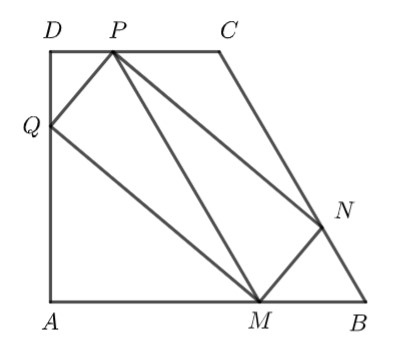
\includegraphics[max width=0.42\textwidth, alt={Правоъгълен трапец ABCD с вписан правоъгълник MNPQ}, center]{assets/7-3-trapezoid.jpeg}

а) Намерете отношението $DP:PC$.

б) Върху отсечката $AM$ е избрана точка $X$ така, че отсечката $AX$ е равна на $37\%$ от $MB$. Пресечната точка на отсечките $PN$ и $MC$ е означена с $E$, а пресечната точка на $PX$ и $MQ$ с $F$. Докажете, че
$$
S_{MEPF}=S_{AXFQ}+S_{MBN}+S_{ENC}+S_{DQP}.
$$

Решение. От $PD=3k$, $DQ=4k$ по Питагорова теорема за триъгълника $DPQ$ получаваме $QP^2=(3k)^2+(4k)^2=(5k)^2$, т.е. $QP=5k$.

Аналогично, от $QA=3n$, $AM=4n$ намираме $QM=5n$.

Тъй като $DQ:QA=3:4$, то
$$
\frac{4k}{3n}=\frac34\Longleftrightarrow k:n=9:16.
$$
Изразяваме $S_{MNPQ}=5k\cdot5n=25kn$ и $S_{MNP}=\dfrac12S_{MNPQ}=\dfrac{25}{2}kn$.

Тъй като $PM$ е успоредна на $BC$ и $AB$ е успоредна на $CD$, то $MBCP$ е успоредник. Тогава
$$
S_{MNP}=\frac12\cdot MP\cdot h_{MP}=\frac12\cdot S_{MBCP}
$$
и получаваме, че $S_{MBCP}=2S_{MNP}=25kn$.

От друга страна, $S_{MBCP}=PC\cdot AD$ и тъй като
$$
AD=4k+3n=4\cdot\frac9{16}n+3n=\frac{21}{4}n,
$$
от равенството $25kn=PC\cdot\dfrac{21}{4}n$ намираме $PC=\dfrac{100}{21}k$. Тогава
$$
DP:PC=3:\frac{100}{21}=63:100.
$$

б) Имаме $AX=37\%MB=37\%PC=37\%\cdot\dfrac{100}{21}k=\dfrac{37}{21}k$.

Равенството
$$
S_{MEPF}=S_{AXFQ}+S_{MBN}+S_{ENC}+S_{DQP}
$$
е еквивалентно на
$$
S_{MNPQ}=S_{AXPD}+S_{MBC}
$$
(получава се, като се прибави към двете страни на равенството $S_{FPQ}+S_{MNE}$). Но

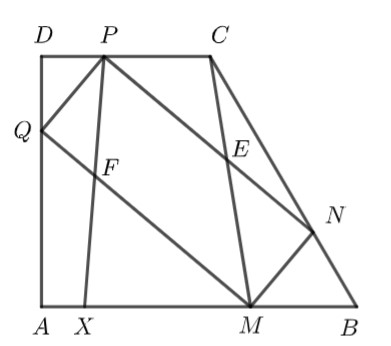
\includegraphics[max width=0.42\textwidth, alt={Трапецът с допълнителните точки X, E и F}, center]{assets/7-3-trapezoid-extended.jpeg}

$$
S_{AXPD}+S_{MBC}=\frac{AX+DP}{2}\cdot AD+\frac{MB}{2}\cdot AD=\frac{AX+DP+MB}{2}\cdot AD=
$$
$$
=\frac12\left(\frac{37}{21}k+3k+\frac{100}{21}k\right)\cdot\frac{21}{4}n=\frac12\cdot\frac{200}{21}k\cdot\frac{21}{4}n=25kn=S_{MNPQ},
$$
което искахме да докажем.

Оценяване. а) Пълно решение: 5 точки.

Изразяване на $PD,DQ,QA,AM$ – 1 точка.

Прилагане на Питагоровата теорема и изразяване на страните и лицето на правоъгълника – 2 точки.

Доказателство, че лицето на успоредника $MBCP$ е равно на лицето на правоъгълника – 1 точка.

Изразяване на $PC$ и намиране на търсеното отношение – 1 точка.

б) Пълно решение: 2 точки.

Свеждане на даденото равенство до $S_{MNPQ}=S_{AXPD}+S_{MBC}$ – 1 точка.

Доказване на това равенство – 1 точка.

Задача 7.4. За редица от нули и единици са разрешени следните действия:

Действие $X$: две поредни цифри 01 се заменят с 10. Например,
$$
1010\xrightarrow{X}1100.
$$
Действие $Y$: две поредни цифри 01 се заменят с 110. Например,
$$
1010\xrightarrow{Y}11100.
$$

a) Започваме от редица $A$, която се състои от 20 цифри (0 или 1), и последователно прилагаме действие $X$:
$$
A\xrightarrow{X}A_1\xrightarrow{X}A_2\text{ и т.н., докато е възможно.}
$$
Най-много колко пъти последователно може да се приложи действие $X$? При коя начална редица $A$ се получава това?

б) Започваме от редица $B$, която се състои от 20 цифри (0 или 1), и последователно прилагаме действие $Y$:
$$
B\xrightarrow{Y}B_1\xrightarrow{Y}B_2\text{ и т.н., докато е възможно.}
$$
Най-много колко цифри може да има в редица, която е получена по този начин?

Решение. а) Нека в редицата $A$ има $a$ цифри 0 и $20-a$ цифри 1.

Към всяка двойка 0 и 1 в $A$ действието $X$ може да се приложи най-много веднъж (защото след това тази нула минава вдясно от единицата). Двойките 0 и 1 в редицата $A$ са $a(20-a)$ на брой. Следователно действието $X$ може да се приложи най-много $a(20-a)$ пъти. Тази стойност се реализира при
$$
A=\underbrace{0\ldots0}_{a}\underbrace{1\ldots1}_{20-a}:
$$
$$
\underbrace{0\ldots0}_{a}\underbrace{1\ldots1}_{20-a}\xrightarrow{X}\underbrace{0\ldots0}_{a-1}10\underbrace{1\ldots1}_{19-a}\xrightarrow{X}\underbrace{0\ldots0}_{a-2}100\underbrace{1\ldots1}_{19-a}\xrightarrow{X}\cdots\xrightarrow{X}
$$
$$
1\underbrace{0\ldots0}_{a}\underbrace{1\ldots1}_{19-a}\xrightarrow{X}\cdots\xrightarrow{X}11\underbrace{0\ldots0}_{a}\underbrace{1\ldots1}_{18-a}\xrightarrow{X}\cdots\xrightarrow{X}\underbrace{1\ldots1}_{20-a}\underbrace{0\ldots0}_{a}.
$$
Броят на действията $X$ в редица с $a$ цифри 0 и $20-a$ цифри 1 е най-много
$$
a(20-a)=100-(a-10)^2\leq100,
$$
т.е. е най-много 100, като тази стойност се достига при $a=10$ и
$$
A=\underbrace{0\ldots0}_{10}\underbrace{1\ldots1}_{10}.
$$

б) Нека вляво от дадена цифра 1 има $k$ цифри 0. Това поражда следните последователни действия $Y$:
$$
\underbrace{0\ldots0}_{k}1\xrightarrow{Y}\underbrace{0\ldots0}_{k-1}110\xrightarrow{Y}\underbrace{0\ldots0}_{k-2}11010\xrightarrow{Y}\underbrace{0\ldots0}_{k-2}111100\xrightarrow{Y}
$$
$$
\underbrace{0\ldots0}_{k-3}11011100\xrightarrow{Y}\underbrace{0\ldots0}_{k-3}111101100\xrightarrow{Y}\underbrace{0\ldots0}_{k-3}1111110100\xrightarrow{Y}
$$
$$
\underbrace{0\ldots0}_{k-3}\underbrace{11111111}_{2^3}000\xrightarrow{Y}\cdots\xrightarrow{Y}\underbrace{1\ldots1}_{2^k}\underbrace{0\ldots0}_{k}.
$$
Ако в редицата има $b$ цифри 0 и $c=20-b$ цифри 1, най-дългата възможна редица е с дължина $c\cdot2^b+b$. Ако увеличим броя на единиците до $c+1$ и нулите станат $b-1$, получаваме максимална дължина $(c+1)\cdot2^{b-1}+b-1$. Тъй като
$$
c\cdot2^b+b=2c\cdot2^{b-1}+b>(c+1)\cdot2^{b-1}+b-1,
$$
следва, че с увеличаване на броя на единиците, максималната дължина на редиците намалява.

Следователно най-дълга редица се получава, когато $c=1$ и $b=19$. Получихме, че с действие $Y$ може да се получи редица с най-много $2^{19}+19$ цифри.

Оценяване. а) Пълно решение: 2 точки.

За посочване на верен отговор за максимален брой ходове – 0,5 точки.

Посочване на примера, при който се достига максимумът – 0,5 точки.

Доказателство – 1 точка.

б) Пълно решение: 5 точки.

За посочване на верен отговор за максималната дължина – 1 точка.

Посочване на примера, при който се достига най-голяма дължина на редицата – 1 точка.

Доказателство – 3 точки.
